\documentclass[crop,tikz]{standalone}%

% \usepackage{tikz}
\usetikzlibrary{matrix,calc,positioning}

\begin{document}

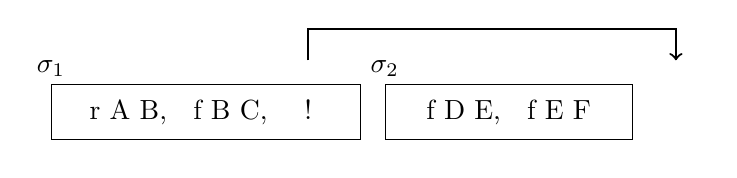
\begin{tikzpicture}[baseline]

\matrix (outer) [matrix of nodes,
                 nodes={draw, minimum width=0.5cm, minimum height=0.7cm, text height=1.5ex, text depth=.25ex, anchor=center},
                 column sep=0.3cm, row sep=0.3cm] {
\phantom{AAAAAAAAAAAAAA} & \phantom{AAAAAAAAAAA} &  \node[draw=none] (A) {\phantom{!}};\\
};

\matrix (inner) [matrix of nodes,
                 nodes={minimum width=0.6cm, minimum height=0.7cm, text height=1.5ex, text depth=.25ex},
                 column sep=0.1cm, row sep=0.1cm] at (outer-1-1.center) {
r A B, & f B C, & ! \\
};

\matrix (inner1) [matrix of nodes,
                 nodes={minimum width=0.6cm, minimum height=0.7cm, text height=1.5ex, text depth=.25ex},
                 column sep=0.1cm, row sep=0.1cm] at (outer-1-2.center) {
f D E, & f E F \\
};


\matrix (inner2) [matrix of nodes,
                 nodes={minimum width=0.6cm, minimum height=0.7cm, text height=1.5ex, text depth=.25ex},
                 column sep=0.1cm, row sep=0.1cm] at (A.center) {
\phantom{x} \\
};

\draw[->, thick]
  ($(inner-1-3.north)+(0,0.3)$) -- ++(0,0.4)
  -- ($(inner2-1-1.north)+(0,0.7)$)         
  -- ($(inner2-1-1.north)+(0,0.3)$);        

\node at ($(outer-1-1.north west)+(-0,0.2)$) {$\sigma_1$};
\node at ($(outer-1-2.north west)+(-0,0.2)$) {$\sigma_2$};
\end{tikzpicture}

\end{document}
